\providecommand{\muc}{\mu_{\mathrm c}}
\providecommand{\mul}{\mu_{\mathrm L}}
\providecommand{\thetac}{\theta_{\mathrm c}}
\providecommand{\thetaL}{\theta_{\mathrm L}}
\providecommand{\varphiL}{\varphi_{\mathrm L}}
\providecommand{\vc}{v_{\mathrm c}}
\providecommand{\Vc}{V_{\mathrm c}}
\providecommand{\bvc}{\mathbf{v}_{\mathrm c}}
\providecommand{\bVc}{\mathbf{V}_{\mathrm c}}
\providecommand{\bVCM}{\mathbf{V}_{\mathrm{CM}}}
\providecommand{\VCM}{V_{\mathrm{CM}}}
\providecommand{\Expect}{\mathbb{E}}
\providecommand{\SourceEq}[1]{\par\nobreak\hfill{\sffamily\scriptsize\color{KSUGray}#1}\par}

\setlength{\abovedisplayskip}{4pt plus 1pt minus 1pt}
\setlength{\belowdisplayskip}{4pt plus 1pt minus 1pt}
\setlength{\abovedisplayshortskip}{3pt plus 1pt}
\setlength{\belowdisplayshortskip}{3pt plus 1pt}
\setlength{\jot}{2pt}
\tcbset{handout base/.append style={before skip=2.5pt,after skip=2.5pt}}

\HandoutSetup
  {NE 630}
  {07}
  {Scattering Kinematics}
  {Textbook \S2.5}

\begin{document}
\MakeHandoutTitle

\textcolor{KSUDeepPurple}{\textbf{Primary objective.}}
Estimate the number of elastic collisions needed to slow a neutron from
$E_0$ to $E_n$ for a target modeled by mass number $A\geq1$.
\par\vspace{5pt}

\begin{handoutcolumns}
\HandoutSection{1}{Review: threshold reactions}

\begin{fixedbox}{Uranium-238 review figure}
\begin{minipage}[c][1.32in][c]{\linewidth}
\centering
\IfFileExists{figures/u238_threshold.pdf}{  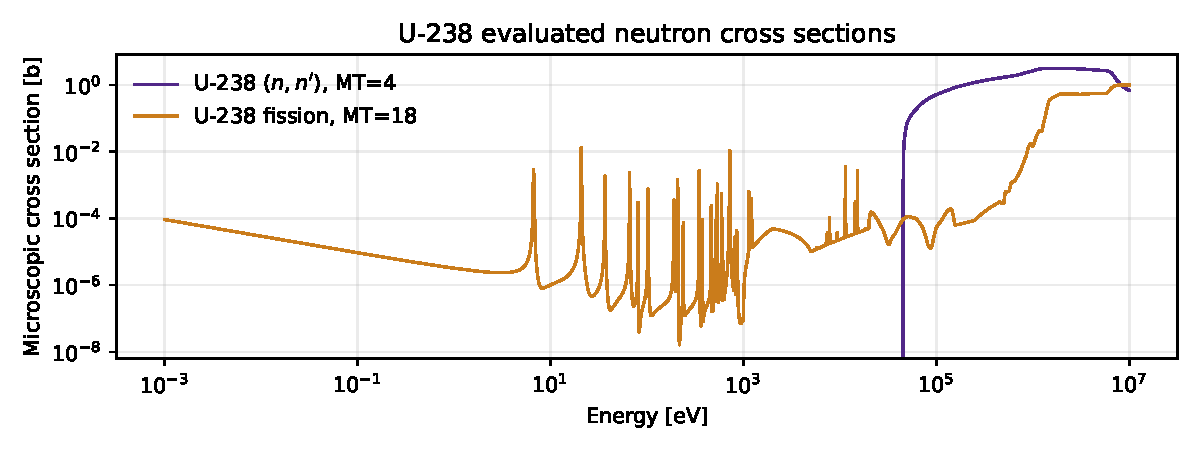
\includegraphics[width=\linewidth,height=1.30in,keepaspectratio]{figures/u238_threshold.pdf}}{  {\sffamily\small\color{KSUGray}Review figure unavailable.\par}
  \vspace{6pt}
  {\ttfamily\footnotesize figures/u238\_threshold.pdf\par}
}
\end{minipage}
\end{fixedbox}

\textbf{Review question.} Do any of these interactions involve
\textbf{threshold} reactions?
\RuledLines{1}

\HandoutSection{2}{Frames and notation}
The target is initially at rest in the \textbf{laboratory} (lab) frame.
Primes denote quantities \emph{after} the collision; a subscript $\mathrm c$
denotes the \textbf{center-of-mass} (CM) frame.

\begin{fixedbox}{Keep the quantities distinct}
\renewcommand{\arraystretch}{1.12}
\begin{tabularx}{\linewidth}{@{}l >{\raggedright\arraybackslash}X@{}}
$m_n,\ M_N$ & Neutron and target masses; $A\equiv M_N/m_n\simeq$ mass number.\\
$\mathbf v,\ \mathbf V$ & Neutron and target velocities in the lab; $\mathbf V=\mathbf0$ initially.\\
$v,\ V$ & Speeds: $v=\|\mathbf v\|$, $V=\|\mathbf V\|$.\\
$\bVCM$ & Velocity of the CM frame relative to the lab.\\
$E,\ E'$ & Incident and outgoing neutron energies in the lab.\\
$\muc,\ \mul$ & $\muc=\cos\thetac$,\quad $\mul=\cos\thetaL$.\\
$\varphiL$ & Target recoil angle in the lab.
\end{tabularx}
\end{fixedbox}

{\centering
{\sffamily\bfseries\footnotesize Laboratory frame}\par\vspace{1pt}
\begin{tikzpicture}[x=1.35cm,y=1.14cm,>=Latex,every node/.style={font=\small}]
  \node[circle,draw,fill=KSUPurple,minimum size=5pt,inner sep=0pt] (a) at (-2,0) {};
  \node[circle,draw,fill=KSUOrange,minimum size=13pt,inner sep=0pt] (b) at (0,0) {};
  \draw[->,shorten <=2pt,shorten >=2pt] (a) -- (b) node[midway,below=2pt] {$\mathbf v$};
  \node[circle,draw,fill=KSUPurple,minimum size=5pt,inner sep=0pt] (c) at (1,1) {};
  \node[circle,draw,fill=KSUOrange,minimum size=13pt,inner sep=0pt] (d) at (1,-1) {};
  \coordinate (e) at (2,0);
  \draw[->,shorten <=2pt,shorten >=2pt] (b) -- (c) node[pos=0.25,above left=2pt] {$\mathbf v'$};
  \draw[->,shorten <=2pt,shorten >=2pt] (b) -- (d) node[pos=0.25,below left=2pt] {$\mathbf V'$};
  \draw[dashed,KSUGray] (b) -- (e);
  \pic[draw,angle radius=8.5mm,->,angle eccentricity=1.52,"$\thetaL$",shorten <=1pt,shorten >=1pt] {angle=e--b--c};
  \pic[draw,angle radius=8.5mm,<-,angle eccentricity=1.52,"$\varphiL$",shorten <=1pt,shorten >=1pt] {angle=d--b--e};
\end{tikzpicture}\par
\vspace{3pt}
{\sffamily\bfseries\footnotesize Center-of-mass frame}\par\vspace{1pt}
\begin{tikzpicture}[x=1.35cm,y=1.14cm,>=Latex,every node/.style={font=\small}]
  \node[circle,draw,fill=KSUPurple,minimum size=5pt,inner sep=0pt] (a) at (-2,0) {};
  \node[circle,draw,fill=KSUOrange,minimum size=13pt,inner sep=0pt] (b) at (2,0) {};
  \coordinate (cm) at (0,0);
  \draw[->,shorten <=2pt,shorten >=2pt] (a) -- (cm) node[midway,above] {$\bvc$};
  \draw[->,shorten <=2pt,shorten >=2pt] (b) -- (cm) node[midway,below] {$\bVc$};
  \node[circle,draw,fill=KSUPurple,minimum size=5pt,inner sep=0pt] (c) at (0.5,1) {};
  \draw[->,shorten <=1pt,shorten >=2pt] (cm) -- (c) node[midway,above left] {$\bvc'$};
  \node[circle,draw,fill=KSUOrange,minimum size=13pt,inner sep=0pt] (d) at (-0.5,-1) {};
  \draw[->,shorten <=1pt,shorten >=2pt] (cm) -- (d) node[midway,below right] {$\bVc'$};
  \pic[draw,angle radius=8.5mm,->,angle eccentricity=1.50,"$\thetac$",shorten <=1pt,shorten >=1pt] {angle=b--cm--c};
\end{tikzpicture}\par
{\sffamily\scriptsize\itshape Schematics; not to scale.}\par}

\switchcolumn
\RaggedRight
\HandoutSection{3}{Conservation and frame changes}
\begingroup\footnotesize
Conservation of momentum and energy in the \textbf{lab} frame requires
\begin{align*}
  m_n\mathbf v &= m_n\mathbf v' + M_N\mathbf V',\\
  \tfrac12m_n v^2 &= \tfrac12m_n v'^2+\tfrac12 M_N V'^2.
\end{align*}
In the \textbf{CM} frame, the corresponding statements are
\begin{align*}
  m_n\bvc+M_N\bVc &= \mathbf0,\\
  m_n\bvc'+M_N\bVc' &= \mathbf0,\\
  \tfrac12m_n\vc^2+\tfrac12M_N\Vc^2
    &=\tfrac12m_n\vc'^2+\tfrac12M_N\Vc'^2.
\end{align*}
Elastic scattering preserves the individual CM speeds:
\[
\vc'=\vc,\qquad \Vc'=\Vc.
\]
The CM velocity and the transformations back to the lab are
\begin{align*}
  \bVCM &=\frac{m_n}{m_n+M_N}\mathbf v
         =\frac{1}{1+A}\mathbf v,\\
  \mathbf v'&=\bvc'+\bVCM,\\
  \mathbf V'&=\bVc'+\bVCM.
\end{align*}
Vector identities, such as
$\mathbf x\!\cdot\!\mathbf y=xy\cos\theta$, connect energies and angles.
\endgroup

\HandoutSection{4}{Elastic-scattering equations}
\begin{fixedbox}{Energy, angles, and the mean lab cosine}
With $E$ and $A$ fixed, $E'$ and $\thetac$ share a one-to-one relationship:
\[
\frac{E'}{E}=\frac{A^2+2A\muc+1}{(A+1)^2}.
\]
\medskip
The lab and CM angles are also linked one-to-one for $A\geq1$
(apart from the endpoint noted below):
\[
\mul=\frac{1+A\muc}{\sqrt{A^2+2A\muc+1}}.
\]
\medskip
For \textbf{isotropic CM scattering}, the average lab cosine is
\[
\overline{\mu}_{\mathrm L}\equiv\Expect[\cos\thetaL]
  =\frac{2}{3A}\qquad(A\geq1).
\]
\end{fixedbox}

{\footnotesize\textit{Endpoint clarification.}
At $A=1$ and $\muc=-1$, $E'=0$; a neutron at rest has no outgoing lab direction.\par}

\begin{checkpoint}[Ponderables]
What values can $E'$ be? $\muc$? $\mul$?
What happens to $\overline{\mu}_{\mathrm L}$ as $A$ grows?
\RuledLines{2}
\end{checkpoint}
\end{handoutcolumns}

\newpage

\begin{handoutcolumns}
\HandoutSection{5}{A quick summary of probabilities}
Let $X$ be a random variable with probability density $p_X(x)$ and
\textbf{support} $x_{\mathrm L}\leq x\leq x_{\mathrm U}$.

\begin{fixedbox}{A probability density}
\[
\int_{x_{\mathrm L}}^{x_{\mathrm U}}p_X(x)\,dx=1,
\]
\[
p_X(x)\geq0\quad\text{for all }x\in[x_{\mathrm L},x_{\mathrm U}],
\]
and $p_X(x)=0$ outside its support.
\end{fixedbox}

For $x_{\mathrm L}\leq a\leq b\leq x_{\mathrm U}$, the \textbf{probability}
that $X\in[a,b]$ is
\[
P(a\leq X\leq b)=\int_a^b p_X(x)\,dx.
\]
The \textbf{expected value} (or ``average'') of a function $f(X)$ is
\[
\Expect[f(X)]\equiv\bar f
  =\int_{x_{\mathrm L}}^{x_{\mathrm U}}f(x)p_X(x)\,dx.
\]
Here $\Expect[\,\cdot\,]$ denotes expectation; $E$ denotes neutron energy.

\HandoutSection{6}{Transforming probabilities}
Probability densities can be transformed from one variable to another.
We write $p_X(x)$ and $p_Y(y)$ for the densities of $X$ and $Y$.

\medskip
Suppose $Y=g(X)$ is a one-to-one, differentiable mapping.
Corresponding probability elements satisfy
\[
p_X(x)\,|dx|=p_Y(y)\,|dy|.
\]

\begin{fixedbox}{Change of variables}
\begin{align*}
 p_Y(y)
  &=p_X\!\left(g^{-1}(y)\right)
    \left|\frac{d g^{-1}(y)}{dy}\right|\\
  &=\left.\left|\frac{dx}{dy}\right|p_X(x)\right|_{x=g^{-1}(y)}\\
  &=\left.\left|\frac{dy}{dx}\right|^{-1}p_X(x)\right|_{x=g^{-1}(y)}.
\end{align*}
\end{fixedbox}

The support of $Y$ is the image of the support of $X$ under $g$.

\begin{checkpoint}[Example: stretch and shift]
Let $X$ be uniform on $[0,1]$ and let $Y=2X-1$.
Then $p_X(x)=1$ for $0\leq x\leq1$ (and zero elsewhere). Find the
transformed density and support:
\[
p_Y(y)=\left|\frac{dx}{dy}\right|p_X(x)
  =\MathBlank[0.55in]{}.
\]
Support of $Y$: \RevealBlank[1.20in]{}; $p_Y(y)=0$ otherwise.
\end{checkpoint}

\begin{boardbox}{Notes: transforming a density}
\RuledLines{6}
\end{boardbox}

\switchcolumn
\RaggedRight
\HandoutSection{7}{Energy loss from collisions}
\textbf{Condition on an elastic collision that is isotropic in the CM frame.}
For incident neutron energy $E$, the outgoing-energy density is

\begin{fixedbox}{Elastic-scattering energy distribution}
\[
p(E'\mid E)\equiv p(E\!\to\!E')=
\begin{cases}
\dfrac{1}{(1-\alpha)E},&\alpha E\leq E'\leq E,\\[4pt]
0,&\text{otherwise},
\end{cases}
\]
\SourceEq{FNRP 2.47}
where
\[
\alpha=\frac{(A-1)^2}{(A+1)^2}.
\]
\SourceEq{FNRP 2.48}
\end{fixedbox}

Here $p(E'\mid E)$ is a \emph{density in outgoing energy}, with $E$ held fixed;
it is not the probability that a collision occurs.

\begin{checkpoint}[Example: expected outgoing energy]
What is the expected outgoing energy $\overline{E'}$ of a neutron of
energy $E$ after an elastic collision with a target of mass ratio $A$?

\medskip
\[
\overline{E'}=\Expect[E'\mid E]=
  \MathBlank[1.35in]{}.
\]
\RuledLines{2}
\end{checkpoint}

\HandoutSection{8}{Slowing-down decrement}
The \textbf{average logarithmic energy loss}, also called the
\textbf{slowing-down decrement}, is

\begin{fixedbox}{Average logarithmic energy loss}
\[
\xi\equiv\Expect\!\left[\left.\ln\frac{E}{E'}\,\right|E\right]
  =1+\frac{\alpha}{1-\alpha}\ln\alpha.
\]
\SourceEq{FNRP 2.54 and 2.56}
{\footnotesize At $\alpha=0$, the limiting value is $\xi=1$.}
\end{fixedbox}

The approximate number of elastic collisions needed to reduce the
neutron energy from $E_0$ to $E_n$ is

\begin{fixedbox}{Collision-count estimate}
\[
n\approx\frac{1}{\xi}\ln\frac{E_0}{E_n}.
\]
\SourceEq{FNRP 2.59}
\end{fixedbox}

\begin{checkpoint}[Example: slowing down in water]
How many collisions are required, on average, to slow a $2\unit{MeV}$
neutron to $1\unit{eV}$ in water?

\medskip
Using the supplied effective, collision-weighted mixture value
$\xi_{\mathrm{water}}=0.93$,
\[
n\approx\frac{1}{0.93}\ln\!\left(\frac{2\times10^6\unit{eV}}{1\unit{eV}}\right)
  \approx\MathBlank[0.48in]{}.
\]
\RuledLines{2}
\end{checkpoint}
\end{handoutcolumns}

\end{document}
